\documentclass{article}
\usepackage{blindtext}
\usepackage{graphicx}
\graphicspath{ {./images/} }
\usepackage[T1]{fontenc}
\usepackage[utf8]{inputenc}

\title{\textbf{Final Report
\\{\Large Memory Diary}}}

\author{Dvir Barzilay - 318751971,\\ Kineret Ruth Nahary - 206903684 \\ \\
Advisor: Dr. Dvir Amit Ze'ev \\
Computer Science Department \\
Ariel University 
}
\date{23 Sep 2019}

\begin{document}
\maketitle
\newpage
\tableofcontents
\newpage
\section{Abstract}
\subsection{Preview}
No matter who we are and the kinds of lives that we live, we all have memories, whether they're good or bad. Regardless, these memories are always worth remembering at some point, because who knows what will happen?
\\
What if we lost all of our memories one day and cannot remember a thing?
\\\\
That is why keeping a journal is so important, even if you think it is silly, it is one way to recall all of the great events and milestones that occurred in your life. All those memories, experiences, are what shape your personality and define who you are today.
\\\\
In the old days, people kept analog journals written in pen and paper. But now we are equipped with smartphones, tablets and other technologies that are an even better way of keeping our memories intact, since we probably have hundreds, or even thousands of photos and videos to relive moments with.\\
Also, people tend to forget the little moments in life, the details of things we experienced that have moved us and influenced us. That is what our app concentrate about.
\subsection{The App Main Focus}
Memory Diary main focus is to develop a place where users can record every cherished moment into their own personal diary, and remember it for the rest of their lives. All their memories will be within reach in the application that acts as their personal diary, so that they can view and add new memories at any given moment.

\section{Introduction}
\subsection{What Is A Personal Diary?}
A personal diary is a record of a person's experiences, thoughts, and/or feelings, excluding comments on current events outside the writer's direct experience. It is a collection of notes that are intended to remain private or to have a limited circulation amongst friends or relatives. Some people call it a "journal".
\subsection{The origin of the word}
The word 'diary' comes from the Latin word 'diarium'. The word journal comes from the same root through Old French word 'jurnal'. The earliest use of the word refers to a book in which a daily record was written was in Ben Jonson's comedy 'Volpone' in 1605.
\subsection{Web Diaries}
As internet access became commonly available, many people adopted it as another medium in which to chronicle their lives with the added dimension of an audience.\\
The internet has also served as a way of bringing previously unpublished diaries to the attention of historians and other readers, such as the diary of Michael Shiner, a 19th-century slave who documented his life in Washington, D.C.\\
Web-based services such as 'Open Diary' (started in October 1998) and 'LiveJournal' (January 1999) soon appeared to streamline and automate online publishing, but growth in personal storytelling came with the emergence of blogs. Recent advances have also been made to enable the privacy of internet diary entries.
\subsection{Diary Apps}
With the popularization of mobile apps, diary or journaling, apps have become available for iOS and Android. Proponents cite the following as primary reasons for journaling with digital applications: Ease and speed of typing; mobile portability; search capabilities; entry location, date, and other metadata from mobile phones; and, tags and other organizational features.\\
Digital diaries also seem tailored towards shorter-form, in-the-moment writing, similar to user engagement with Facebook, Twitter, Instagram, and other social media services.

\section{App Features}
Memory Diary allows the user to create memories that have descriptions of his thoughts and pictures he can upload to his personal diary, share a memory with other people that had been a part of his experience and get access to his diary no matter where he is at.\\
All these things are achieved by the following features:
\subsection{Cloud Backup}
Today all apps are enabling a Cloud Backup option for their users, in order to keep their data safe and protected from losing it through a natural disaster or malicious software.\\
That is why we have chosen to let our users save their data via cloud backup and not locally on their phone storage, in order for them to be able to access it through any device they want. For that we used Firebase Cloud Storage System.
\subsubsection{Firebase Cloud Storage}
Firebase Cloud Storage System is a powerful, simple, and cost-effective object storage service built for Google scale. The Firebase SDKs for Cloud Storage add Google security to file uploads and downloads for Firebase apps, regardless of network quality. SDKs can be used to store images, audio, video, or other user-generated content. On the server, Google Cloud Storage can be used to access those same files.\\
Firebase Cloud Storage use is a basis for developing additional user interfaces later on, in order to access to his personal diary, be it through browser, desktop, iOS or android application. None of this would have been possible if the user's data was only locally stored on his smartphone.\\ 
Every time the user will add a new memory to his diary, it will be uploaded directly to the cloud storage and will be able to access it through every device in which he will log into his account.
\subsection{Tagging A Friend}
The application supports sharing a certain memory to a contact via phone number. The user can send a copy of a specific memory he has in his diary to an acquaintance of his, be it someone who had been with him and experienced the same things as him or else. The acquaintance will receive a cloned version of the memory and will be able to chose between deleting it or accepting it. Upon acceptance, the memory will be added to his own diary without any connection to the original, so he could edit it as he have experienced it.\\ 
For example, on a family trip abroad, the brothers went trekking and took pictures in places they visited and stopped to sleep. One of the brothers wrote a memory about it in his diary and shared it with the others so they could choose whether to add it to their own diaries.
 \subsubsection{Different from other apps}
 Unlike other apps, our app is not social, it is unlike Facebook or Instagram where everyone can comment on a post or share it. Our app keeps the user's diary private and lets him decide to share something with a specific person - as a shared memory of them both.

\subsection{Advanced Search}
In this feature we have used tools and technologies to gain experience working with tools and technologies. The great challenge in working with a variety of tools designing the system and enabling it to work in collaboration with these tools and technologies, in order to accomplish the task as required. To explain the advanced search development process, we will first review the tools and technologies we used.
\subsubsection{Algolia}
\paragraph{Why use Angolia?}
Algolia is a technology that provides cloud services for creating search engines. Using Algolia allows us to set up a stable, fast and customized search engine for our system needs. We run and configure our entire search engine in Algolia. 
\paragraph{Our use of Algolia}
At the beginning of the process, we had to index all the memories of all the app users. The index consists of documents, each document representing the memory of a certain user. The document contains fields such as the user ID that uploaded the memory, the date the memory was created, the title, the description of the experience, the list of entities identified in the image, and of course the ID number of the memory itself within the index. We had to configure the index and define which fields are searchable or filterable.\\
One of the biggest risks we had to fix was a search engine security breach, where a user could search for memories that didn't belong to him, just because all the memories were within one common index. Therefore, each time a user enters a query, we filter the documents by the field that specifies the memory owner ID. Access to the search engine we created and configured in Algolia was done through appropriate APIs, that allowed us to easily interface with the system.
\subsubsection{Google Cloud Platform (GCP)}
\paragraph{What is GCP?}
GCP is a platform that provides cloud services to the public that drive, among other things, Google's search engine and YouTube. Google's cloud platform provides developers with various products and services, to build a variety of applications and websites from simple to complex.
\paragraph{Our use of GCP}
In our app, we used Google's cloud platform to make use of the products it provides, like well-trained learning machines. Using Google Learning Machines saved us the hassle of designing and developing our own learning machine, which would have probably require a lot of training and would have not allow us to focus on developing the app itself.
\subsubsection{Cloud Vision API}
Google Cloud's Vision API offers powerful pre-trained machine learning models through REST and RPC APIs. Those APIs assign labels to images and quickly classify them into millions of predefined categories, detect objects and faces, read printed and handwritten text, and build valuable metadata into our image catalog.\\
The use of a Google-trained image recognition machine was essential for the advanced search development, as will be explained later.
\subsubsection{Cloud Functions for Firebase}
Cloud Functions for Firebase lets us automatically run backend JavaScript code (Node.js) in response to events triggered by Firebase features, like Firebase Cloud Storage. Our code is stored in Google's cloud and runs in a managed environment.\\
We needed this service for communicating between the tools and enabling collaboration between them, to provide the user with an advanced and high quality search experience as will be explained later.
\subsubsection{Integration}
The advanced search development process required using all the tools, products and services mentioned above. Advanced search has its ability to produce as relevant query results as possible. We saw as a primary goal the need to identify entities in the images that users upload with their memories, to allow the search to return results to queries, even if they do not contain a word for word that users have written explicitly in their memories. The ability to recognize the content displayed in the image, whether it is an object or handwritten text, and the ability to require advanced machine learning skills and the power to search using a fast and stable search engine specifically tailored to these system needs, made this feature complex and advanced.
\\\\
To identify the content displayed in the image, each time the user creates a new memory or an existing memory editor, the application sends a request to GCP servers and they run the Cloud Vision API services to find all the entities identified in the image. In response, the Cloud Vision API returns to the app a list of labels that describe the image content. When the user uploads the memory to their calendar, the memory is sent to Firebase Cloud Storage, and stored there, among other things, for backup purposes.\\\\
Since we chose to use Algolia to run the search engine, we had to make sure that every change made in the user's log also indexed the search engine.
Imagine a situation where you erase memory from the journal but it nevertheless appears when you search for it. Therefore, we have written code in JavaScript language that will be stored on Google servers and run there as soon as a user's log is changed. It was important to us that our code should run on Google's servers, as they had to provide sufficient computing power and bandwidth to suit the number of users who would use the app and run an event that required code execution.\\\\
The use of Node.js was necessary to achieve these goals. Each time a log of one of Firebase Cloud Storage users logs, a dedicated function that interfaces with Algolia is created and the relevant update is updated in the appropriate document in the memory index. That way, we kept our search engine up to date and up to date. The process of memory generation as a whole can be seen in the following sequence diagram:
\\\\
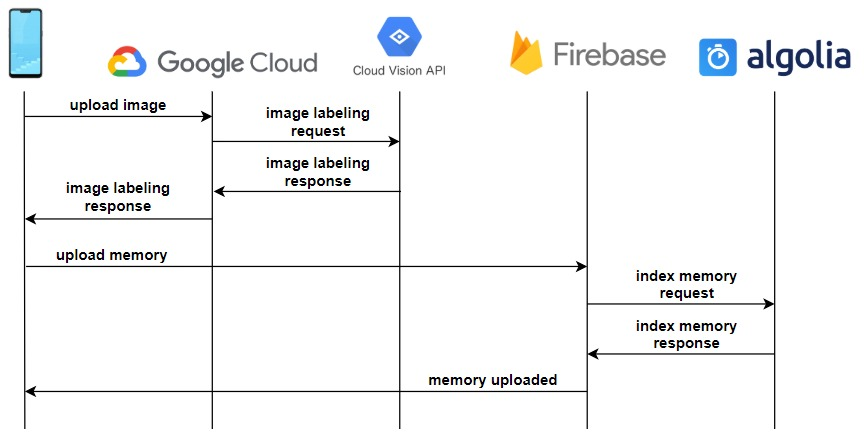
\includegraphics[width=13cm, height=7cm]{uploadMemoryDiagram}
\\\\
In the second part of the advanced search development, we had to develop a user-friendly interface for entering a query, displaying its results, and of course interfacing with Algolia every time the query was written. We have done the UGG interface and interface with Android 'InstantSearch', which is optimized for realizing search for Android apps with the search engine managed in Algolia. This process is also shown in the sequence diagram in front of you:
\\\\
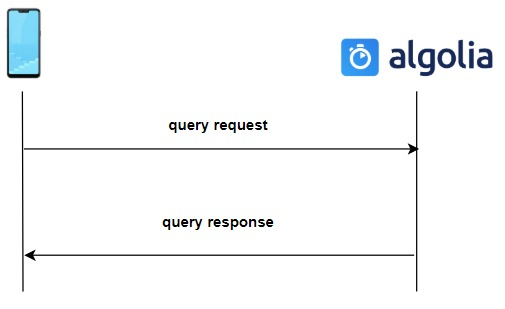
\includegraphics[width=8cm, height=5cm]{searchQueryDiagram}
\\\\
We made most of this feature in Kotlin language, not Java, for the challenge of experimenting with a more innovative and advanced language specifically developed for Android app development and is generally recommended over the use of Java language.
\subsection{Smart Notification System}
The system detects diagnostically a repetitive pattern in the user's daily life, notices and notifies him about unusual events so that the user will remember to record it in his diary.
\subsubsection{Gallery growth analysis}
Once the user first logged to the app, the system analyses once a week, the amount of photos taken in a day and calculates the average. Then, every time the user goes above average, the system interprets it as a possible new memory to document and notifies him of it.
For example, the user goes out on a trip and takes more photos than usual with his phone, the system will notice this change and send a notification asking him if he wants to document something in his diary.

\section{Instructions}
\subsection{Getting Started}
First the user need to insert a user name and his phone number. Then, an SMS message will be sent to his phone, containing a confirmation code that he will need to enter manually or his phone will automatically insert it.
\\\\
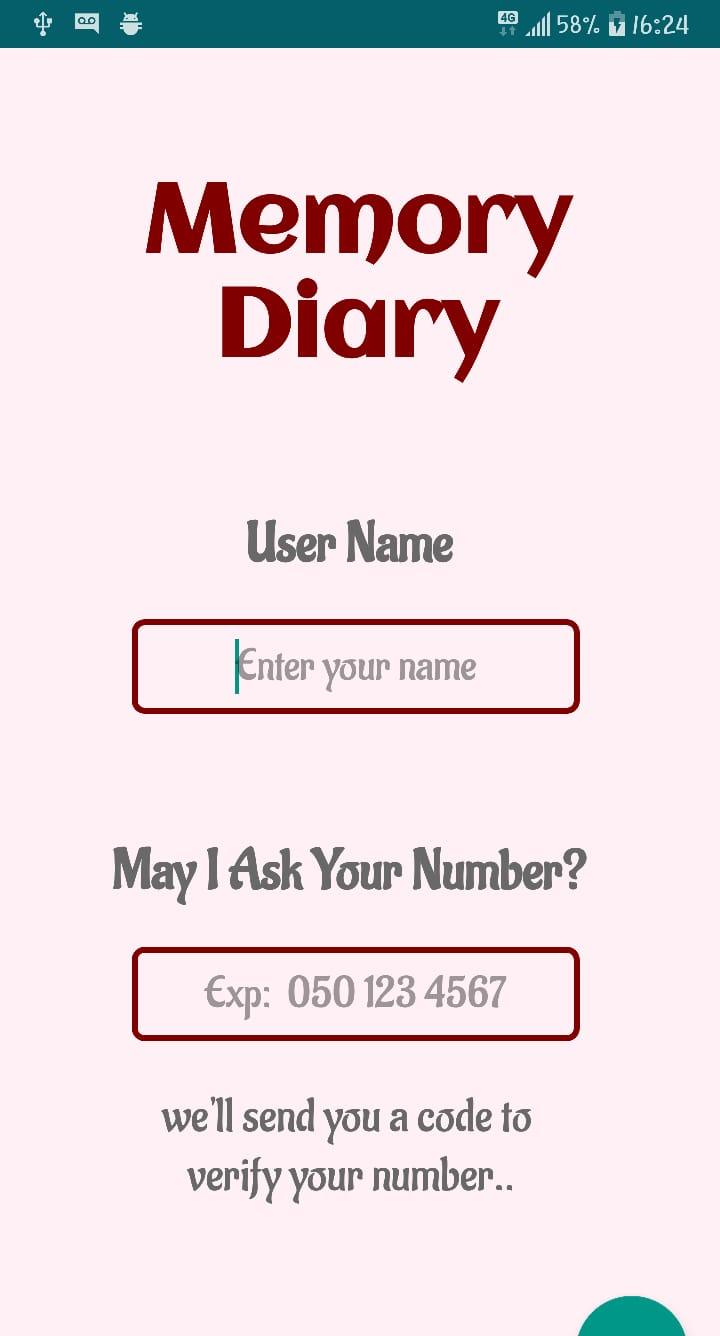
\includegraphics[width=3cm, height=5cm]{register} \quad 
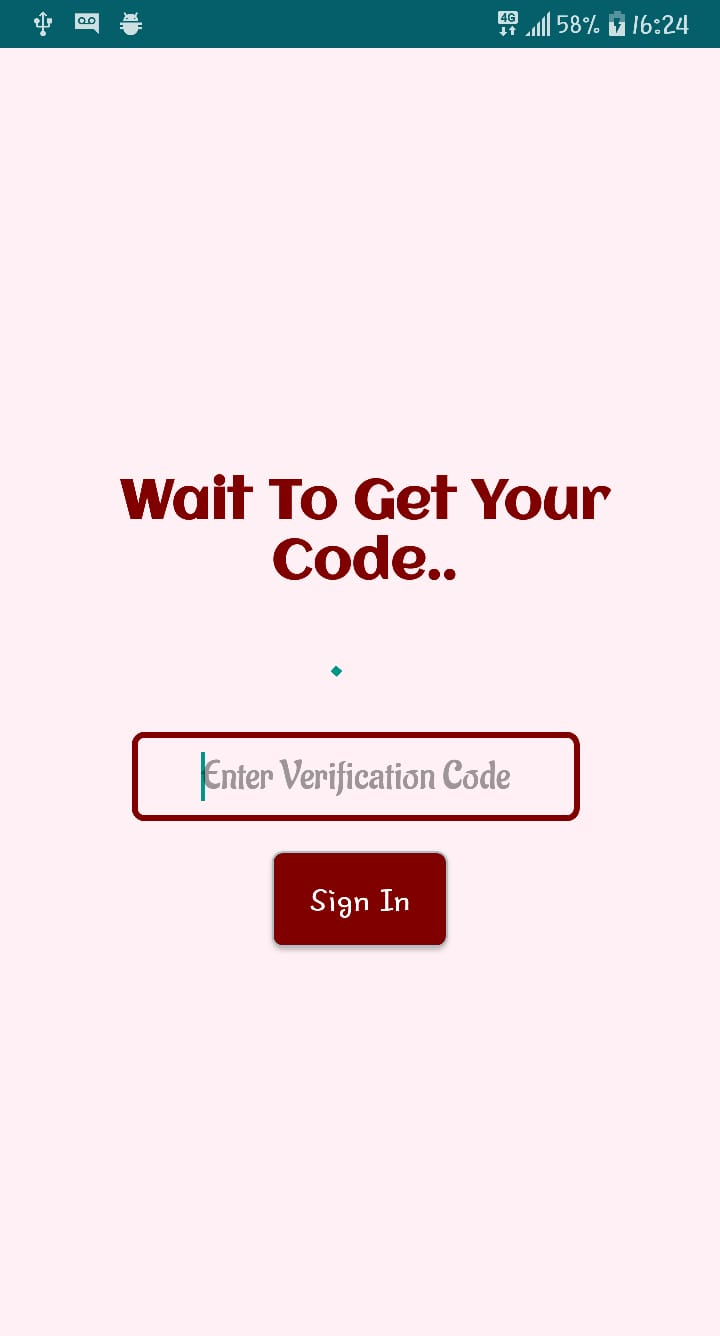
\includegraphics[[width=3cm, height=5cm]{verifyCode}\\
{\small(taken on LG G6-H870)}
\\\\
The user can use the app camera to take photos and upload them to the memory or choose from his gallery. The memory will contain a title, a chosen image and a description of the user experiences and thoughts. Upon submitting the memory he created, it will be added to his diary.
\subsection{Permissions}
After registering to the app, the user  will be asked to give permission to access the phone storage and user the camera.
\\\\
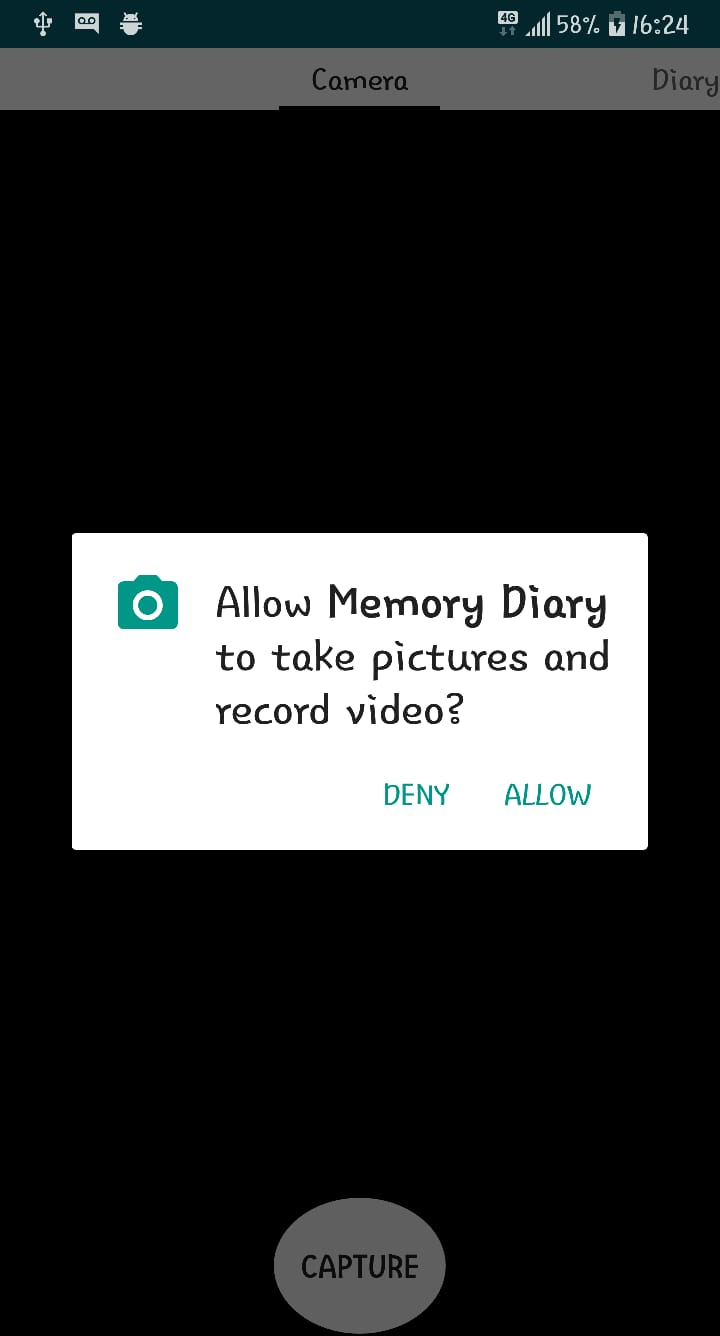
\includegraphics[width=3cm, height=5cm]{permissions}\\
{\small(taken on LG G6-H870)}
\\\\
If not, the user will have to manually give access to this in the phone's settings.
\\\\
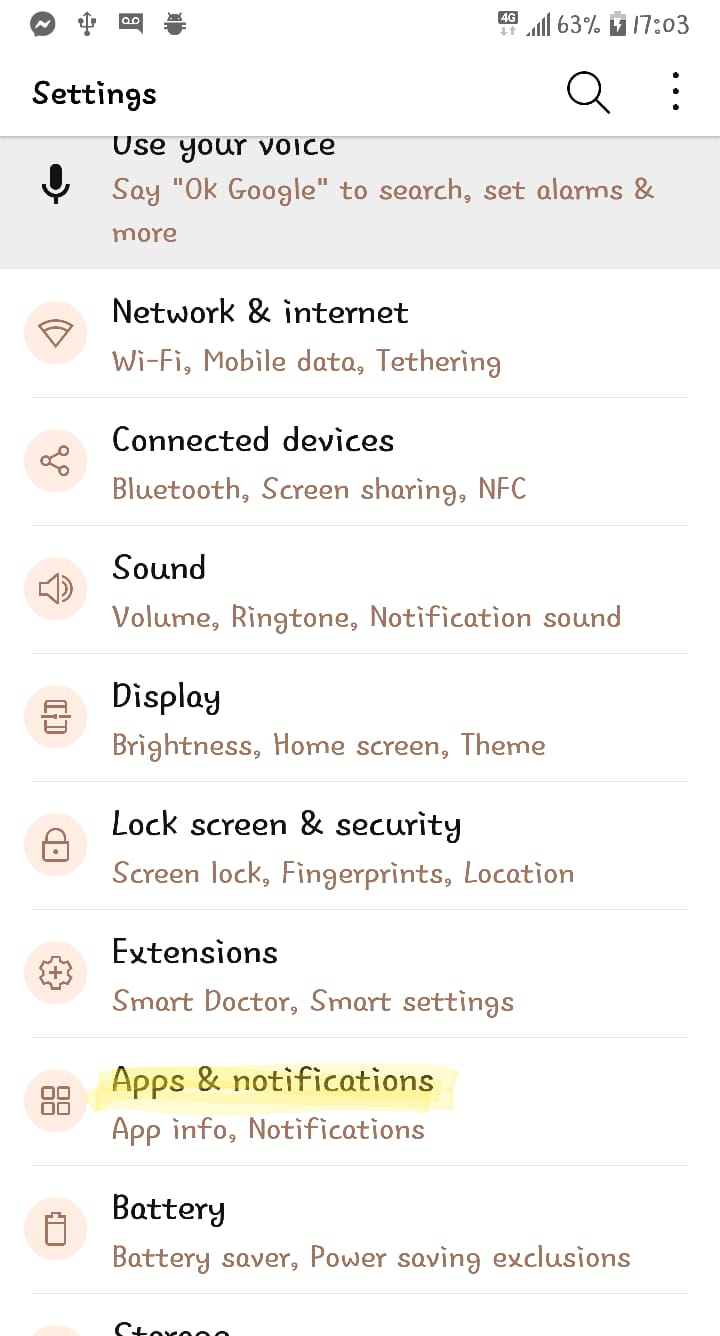
\includegraphics[width=3cm, height=5cm]{permissions2}\quad 
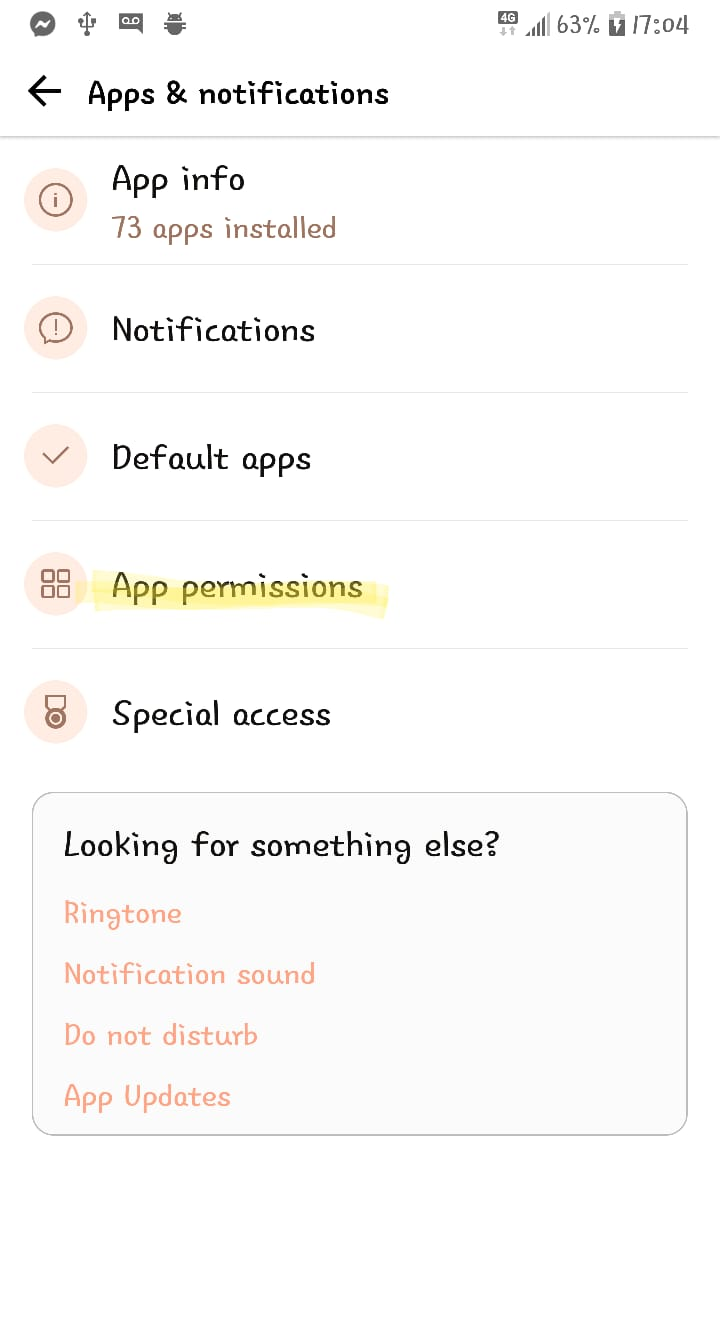
\includegraphics[width=3cm, height=5cm]{permissions3}\\
{\small(taken on LG G6-H870)}
\subsection{Sharing A Memory}
The user can share a selected memory with someone from his contacts. He will need to press a specific memory and choose the 'share' option, then his contacts list will appear and he can select who he wants to share it with. The user will be asked to confirm everything before sending it.
\\\\
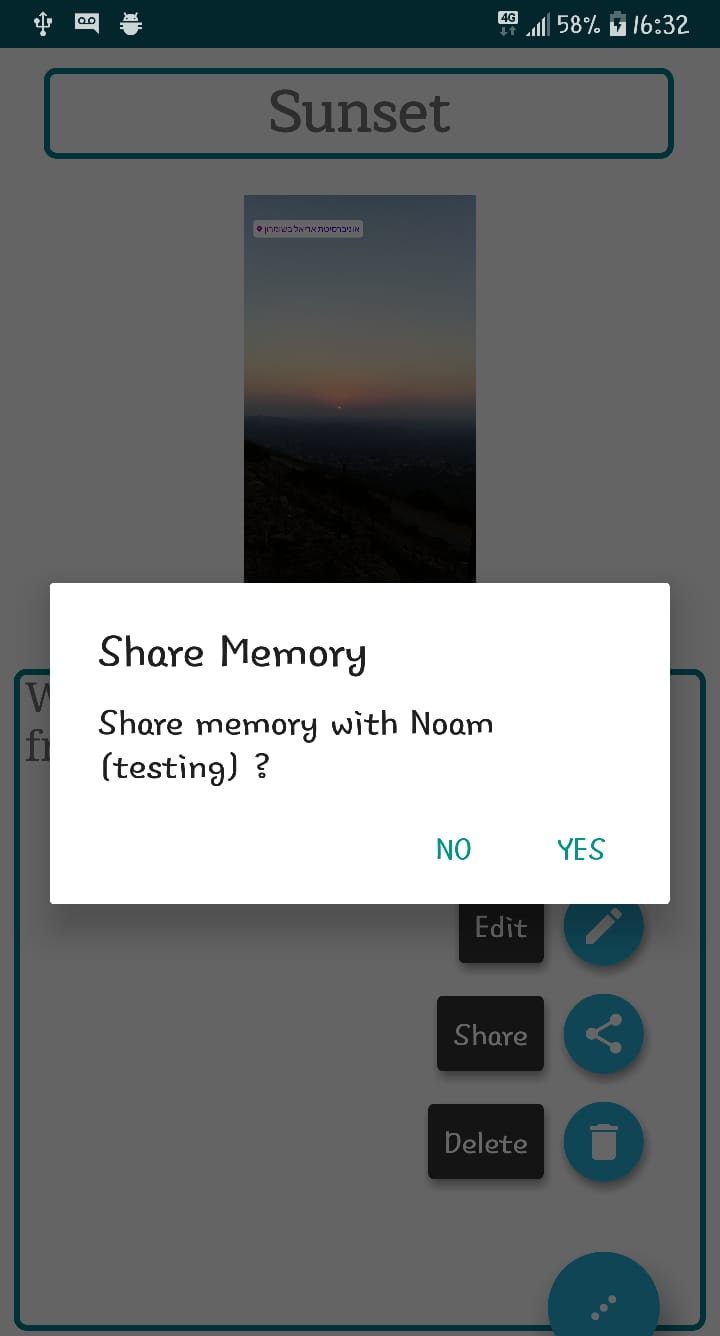
\includegraphics[width=3cm, height=5cm]{shareMemo}\\
{\small(taken on LG G6-H870)}
\\\\
The selected contact will receive a duplicated copy of the memory under the label 'Tags'. He can choose whether to add it to his diary or ignore it by pressing 'delete'.
\\\\
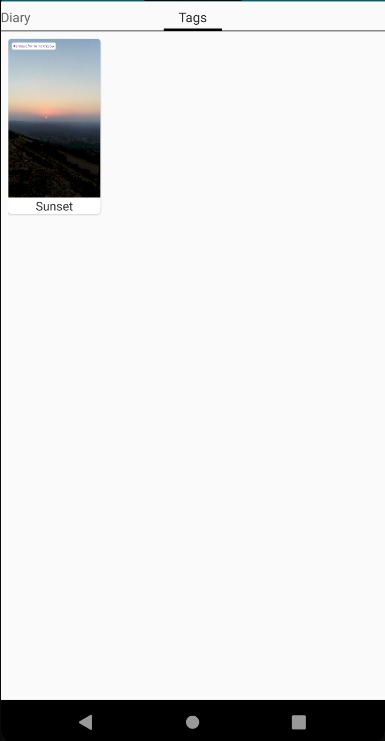
\includegraphics[width=3cm, height=5cm]{sharedMemo1}\quad
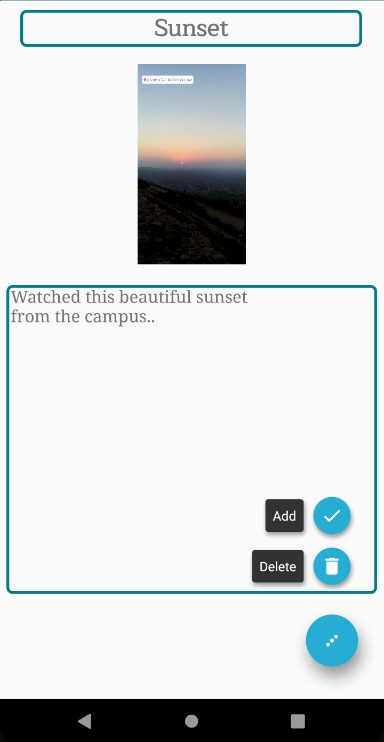
\includegraphics[width=3cm, height=5cm]{sharedMemo2}\\
{\small(taken on Pixel 3 XL)}
\\\\
\subsection{Search In Diary}
Under the label 'Diary' there is an option near the 'search' icon, to search memories that contain specific words or words that describe the images in the memories.
\\\\
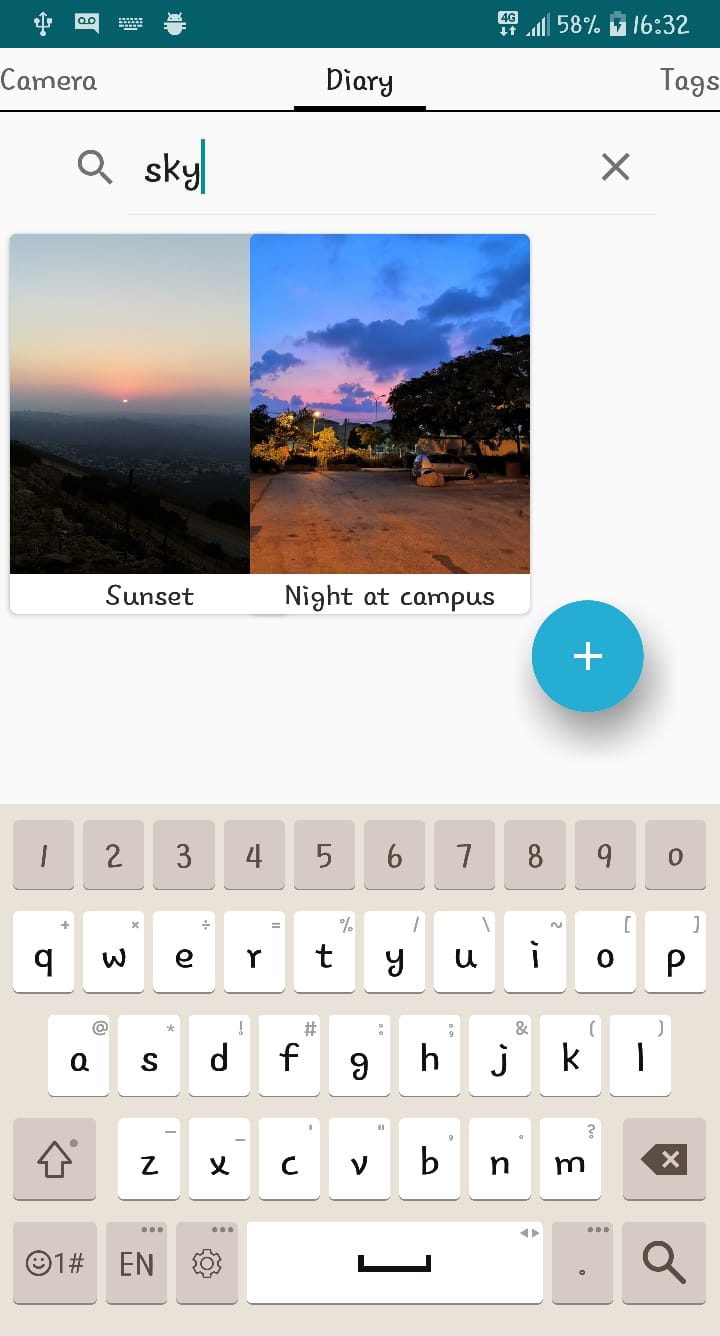
\includegraphics[width=3cm, height=5cm]{searchDiary}\\
{\small(taken on LG G6-H870)}
\\\\
\subsection{Delete Account}
If for some reason the user will want to stop using the app and delete every record of his diary and account, he can go to 'settings' and select the option 'delete account'. Everything including his memories, images and phone number will be erased from the database and storage.

\section{Overall}
So far we have been able to develop a diary application that supports the features we have committed to, but we also believe in further growth in order to create an aspiring application.
\subsection{Features Accomplished}
Currently, the app supports the following features:
\begin{itemize}
 \item Using Firebase to authenticate users (register, log-in, log-out and password recovery).
 \item Uploading a memory to the user's personal diary.
 \item Viewing all user's memories in a Grid layout.
 \item Interfacing the camera when opening the application.
 \item UX (user experience).
 \item Interfacing with GCP (Google Cloud Platform).
 \item Advanced search in the user's memories that includes matching search words to the image content.
\item A cloud backup of the user's diary to have the opportunity to restore data.
\item Tagging friends in memories, thus sharing the data with another user.
\item A smart notification system that reads changes in Gallery and alerts once it goes over the average per day.
\end{itemize}

\subsection{Aspirations For The Future}
We would like the app to support the following features:
\begin{itemize}
\item A smart notification system that gets information about the user location to notify when he is traveling long distance. Also, gets information from various sports and health apps for logging a drastic change in his regular activity.
\item Developing additional user interfaces so that you can view and edit your personal log also through the browser, desktop application or iOS app.
\item Improving UX.
\end{itemize}
\end{document}
